\section{Results}
\label{sec:results}

\begin{figure}[htbp]
	\centering
	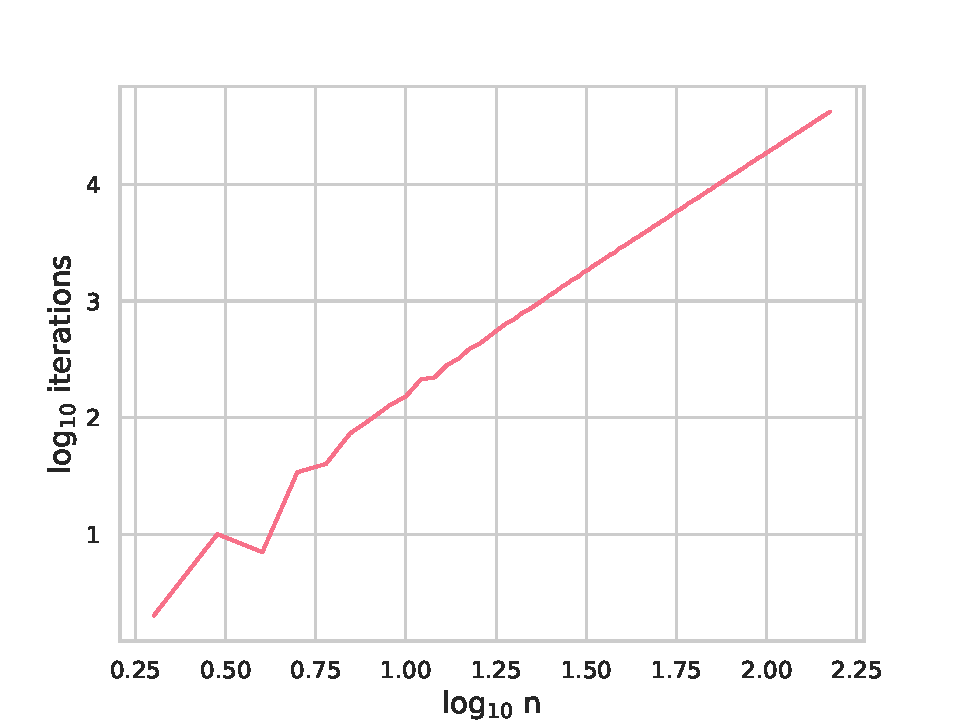
\includegraphics[width=0.5\textwidth]{n_vs_itterations.pdf}
	\caption{Number of iterations used for solving the buckling beam as a function of the matrix dimension n with a logarithmic scale. The slope of the linear fit is 2.11.}
	\label{fig:n_vs_it}
\end{figure}

\begin{figure}[htbp]
	\centering
	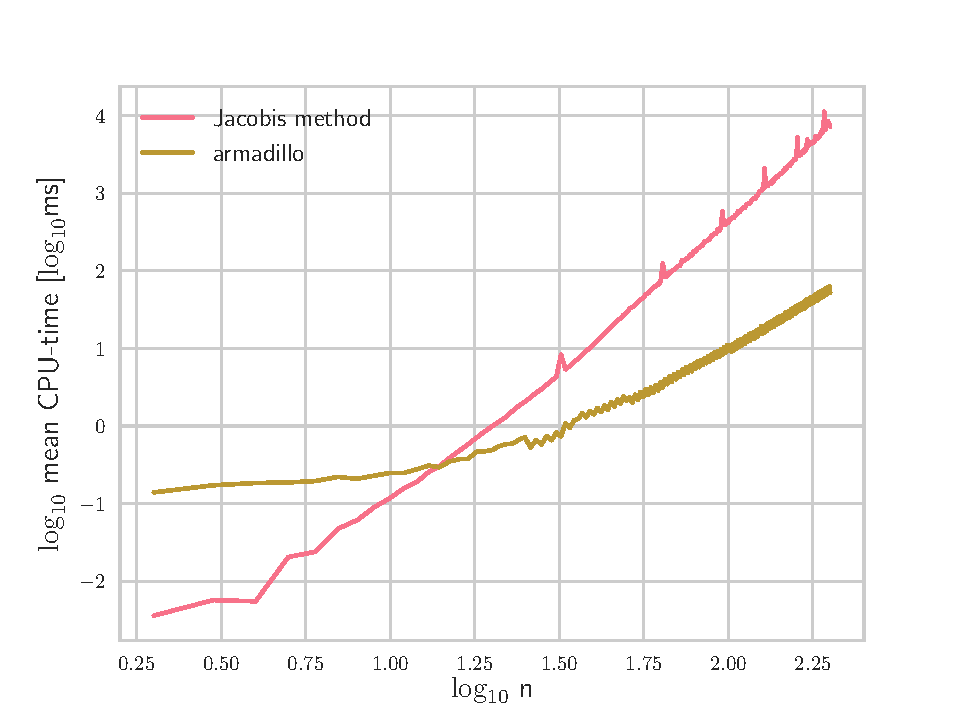
\includegraphics[width=0.5\textwidth]{CPU_time.pdf}
	\caption{CPU time in ms for solving the buckling beam as a function the matrix dimension n. Both Jacobi's method and armadillo's \texttt{eig\_sym} function is shown. The scale is logarithmic.}
	\label{fig:CPUtime}
\end{figure}

\begin{figure}[htbp]
	\centering
	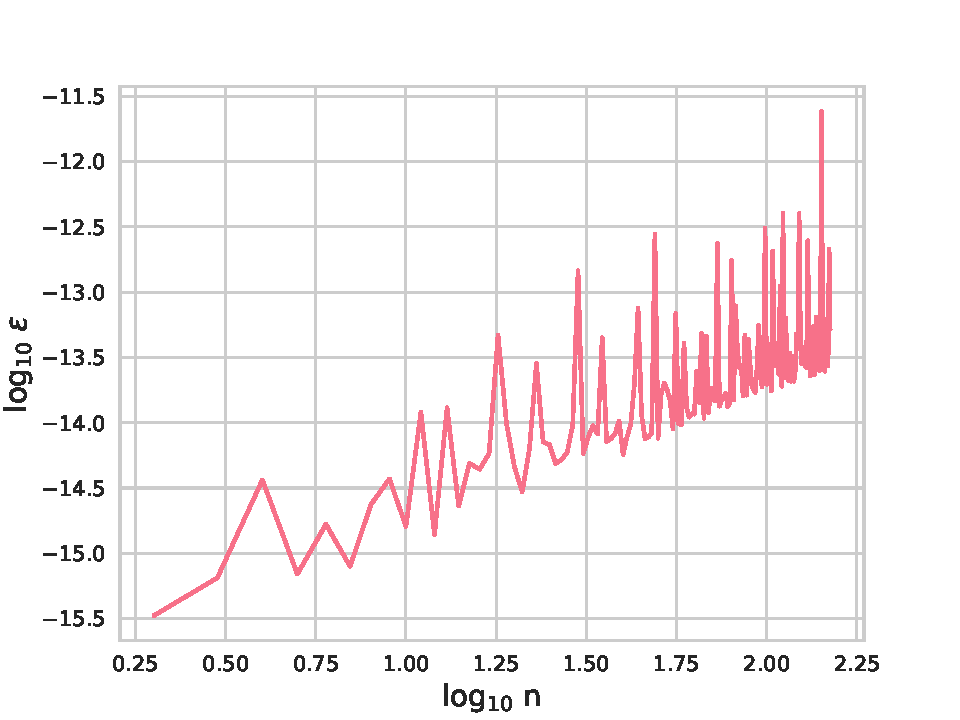
\includegraphics[width=0.5\textwidth]{relative_error.pdf}
	\caption{}
	\label{fig:error}
\end{figure}

